\section{Analyse}

\subsection{Performance}

Der Durchschnitt bei 50 Philosophen:

\begin{verbatim}
CONTAINER ID   NAME                 CPU %     MEM USAGE / LIMIT     MEM %     NET I/O           BLOCK I/O   PIDS
dcd773919aad   vsp-cutlery-3        0.00%     1.641MiB / 30.51GiB   0.01%     145kB / 127kB     0B / 0B     14
898fefa009b1   waiter               0.00%     2.789MiB / 30.51GiB   0.01%     4.42MB / 4.33MB   0B / 0B     13
faff8eb1e008   vsp-philosopher-19   0.00%     1.824MiB / 30.51GiB   0.01%     206kB / 188kB     0B / 0B     14
\end{verbatim}

\subsection{Effizienz}

Feste Konstanten:
\begin{itemize}
    \item Zeit Thinking: 2.00s
    \item Zeit Eating: 2.00s
    \item Zeit Sleeping pro Versuch: 0.01s
\end{itemize}

\subsubsection{Gerade Anzahl an Philosophen}

\begin{table}[h!]
\centering
\begin{tabular}{|c|c|c|c|c|c|c|}
\hline
Anzahl & Eating Avg & Eating Max & Hungry Avg & Hungry Max & Thinking Avg & Thinking Max \\
\hline
4 & 2.01 & 2.04 & 0.13 & 2.14 & 1.99 & 2.00 \\
10 & 2.02 & 2.04 & 0.14 & 2.15 & 1.98 & 2.00 \\
30 & 2.03 & 2.03 & 0.17 & 2.25 & 1.98 & 2.03 \\
50 & 2.02 & 2.04 & 0.17 & 2.25 & 1.99 & 2.04 \\
100 & 2.09 & 2.11 & 0.21 & 2.36 & 1.96 & 2.08 \\
\hline
\end{tabular}
\caption{Performance Daten (Gerade Zahlen)}
\label{tab:performance_data_even}
\end{table}

\begin{figure}[h!]
\centering
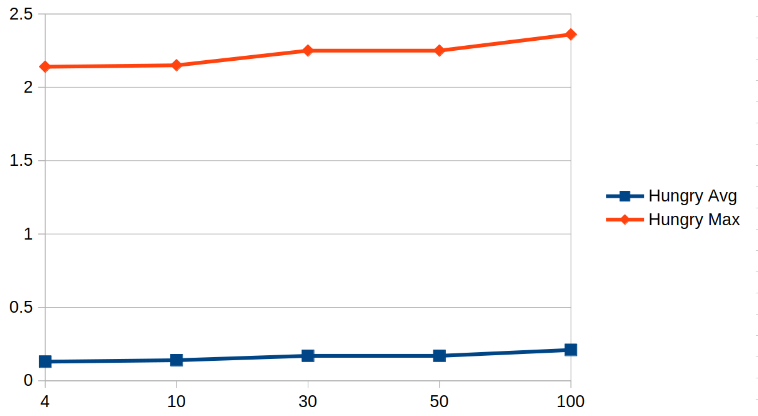
\includegraphics[width=0.8\textwidth]{images/Gerade_Hungry.png}
\caption{Hungry Time bei gerader Anzahl an Philosophen}
\label{fig:gerade_hungry}
\end{figure}

\begin{figure}[h!]
\centering
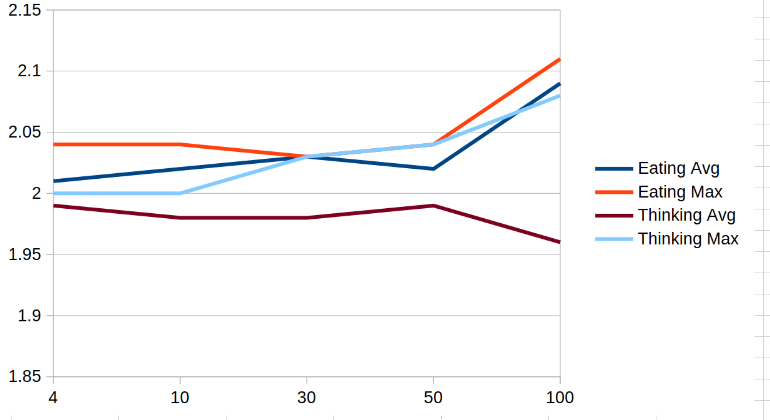
\includegraphics[width=0.8\textwidth]{images/Gerade_Stats.png}
\caption{Statistiken bei gerader Anzahl an Philosophen}
\label{fig:gerade_stats}
\end{figure}

\subsubsection{Ungerade Anzahl an Philosophen}

\begin{table}[h!]
\centering
\begin{tabular}{|c|c|c|c|c|c|c|}
\hline
Anzahl & Eating Avg & Eating Max & Hungry Avg & Hungry Max & Thinking Avg & Thinking Max \\
\hline
5 & 2.01 & 2.04 & 1.18 & 4.17 & 1.98 & 2.00 \\
15 & 2.02 & 2.04 & 0.43 & 4.19 & 1.98 & 2.00 \\
31 & 2.02 & 2.05 & 0.30 & 4.18 & 1.97 & 2.02 \\
51 & 2.04 & 2.06 & 0.26 & 4.29 & 1.97 & 2.04 \\
101 & 2.06 & 2.07 & 0.22 & 4.40 & 1.97 & 2.07 \\
\hline
\end{tabular}
\caption{Performance Daten (Ungerade Zahlen)}
\label{tab:performance_data_odd}
\end{table}

\begin{figure}[h!]
\centering
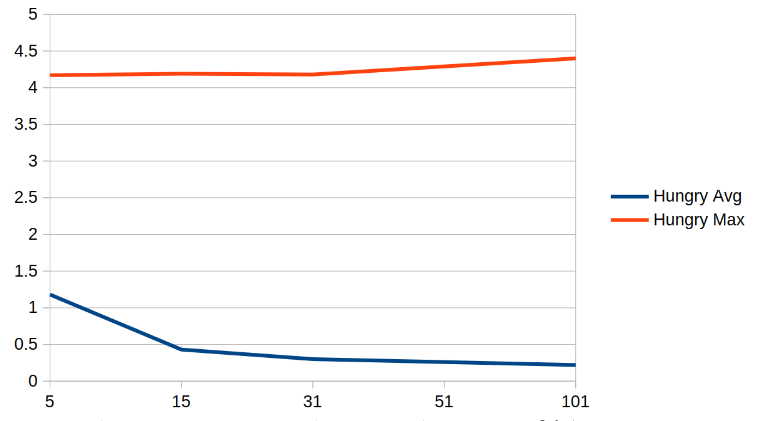
\includegraphics[width=0.8\textwidth]{images/Ungerade_Hungry.png}
\caption{Hungry Time bei ungerader Anzahl an Philosophen}
\label{fig:ungerade_hungry}
\end{figure}

\begin{figure}[h!]
\centering
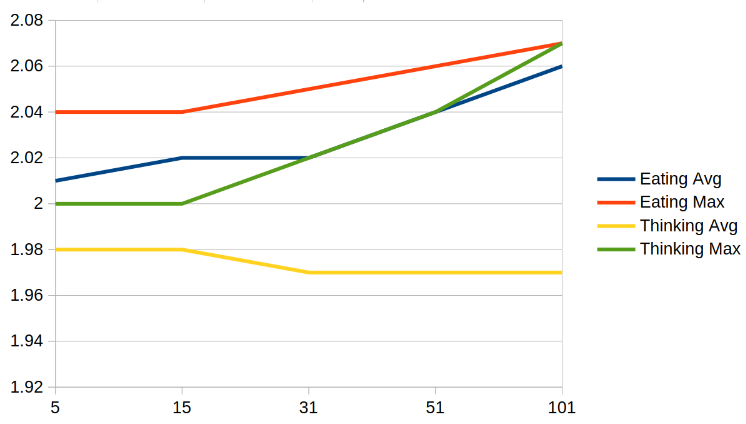
\includegraphics[width=0.8\textwidth]{images/Ungerade_Stats.png}
\caption{Statistiken bei ungerader Anzahl an Philosophen}
\label{fig:ungerade_stats}
\end{figure}

\section{Fazit}

Wir sind mit dem Ergebnis zufrieden, da wir die Anforderungen erfüllt haben und das System effizient und performant ist.

Rust hat sich als eine sehr gute Wahl für das Projekt erwiesen. Jeder Container hat eine sehr niedrige Auslastung und die Kommunikation zwischen den Containern ist sehr effizient 
auf Grund der asynchronen Kommunikation.

Eine der besten Designentscheidungen war es ein "shared_menu" für die verschiedenen Anwendungen zu verwenden,
diese geteilte Bibiliothek erlaubt relativ wenig Code Duplikation und eine einfache Wartung, was sich vorallem bei der Implementierung des RPC Systems bemerkbar gemacht hat.

Dadurch ist z.B. Cutlery unter 100 Zeilen, wovon die größte Menge an Code sehr simple Getter und Setter sind.

Im Laufe des Projektes mussten wir auf Grund von frühen Designentscheidungen einige Änderungen vornehmen, die großes Refactoring benötigten.
Unter anderem das RPC System, welches wir komplett neu geschrieben haben, um Transparenz zu gewährleisten und die Kommunikation zu vereinfachen.

Ein andererer großer Fehler war, wie die Teilnehmer übertragen wurden, 
jeder Teilnehmer hatte eine Kopie von allen anderen Teilnehmern, wodurch die Paketgröße bei vielen Teilnehmern zu groß wurde. 
Nachdem wir nur noch die Nachbarn übertragen haben sehen wir eine deutliche Verbesserung.

Unsere größte Schwachstelle ist der Waiter, dieser ist ein Single Point of Failure und kann das gesamte System zum Stillstand bringen.

Falls wir dieses Projekt in der Zukunft weiterführen würden, würden wir den Waiter etwas mehr dezentralisieren. 

Dazu könnte man den Waiter in mehrere Knoten aufteilen, die sich gegenseitig über ihre Nachbarn informieren
und einen Leader wählen, der für die anfängliche Registrierung zuständig ist.

Nachdem alle Philosophen und Bestecke registriert sind ist die Funktion des Waiters nur noch Logging und Statistiken sammeln, 
was sich gut auf mehrere Knoten aufteilen lässt.